\newenvironment{tmpfigure}
  {\venueifelse{\begin{figure}[H]}{\begin{figure}[H]}}
  {\end{figure}}


\begin{tmpfigure}
    \centering
    \venueifelse{\vskip -0.75\baselineskip}{\vskip -0.25\baselineskip}
    \vskip -0.75\baselineskip
    \begin{subfigure}[t]{0.7\textwidth}
        \centering
        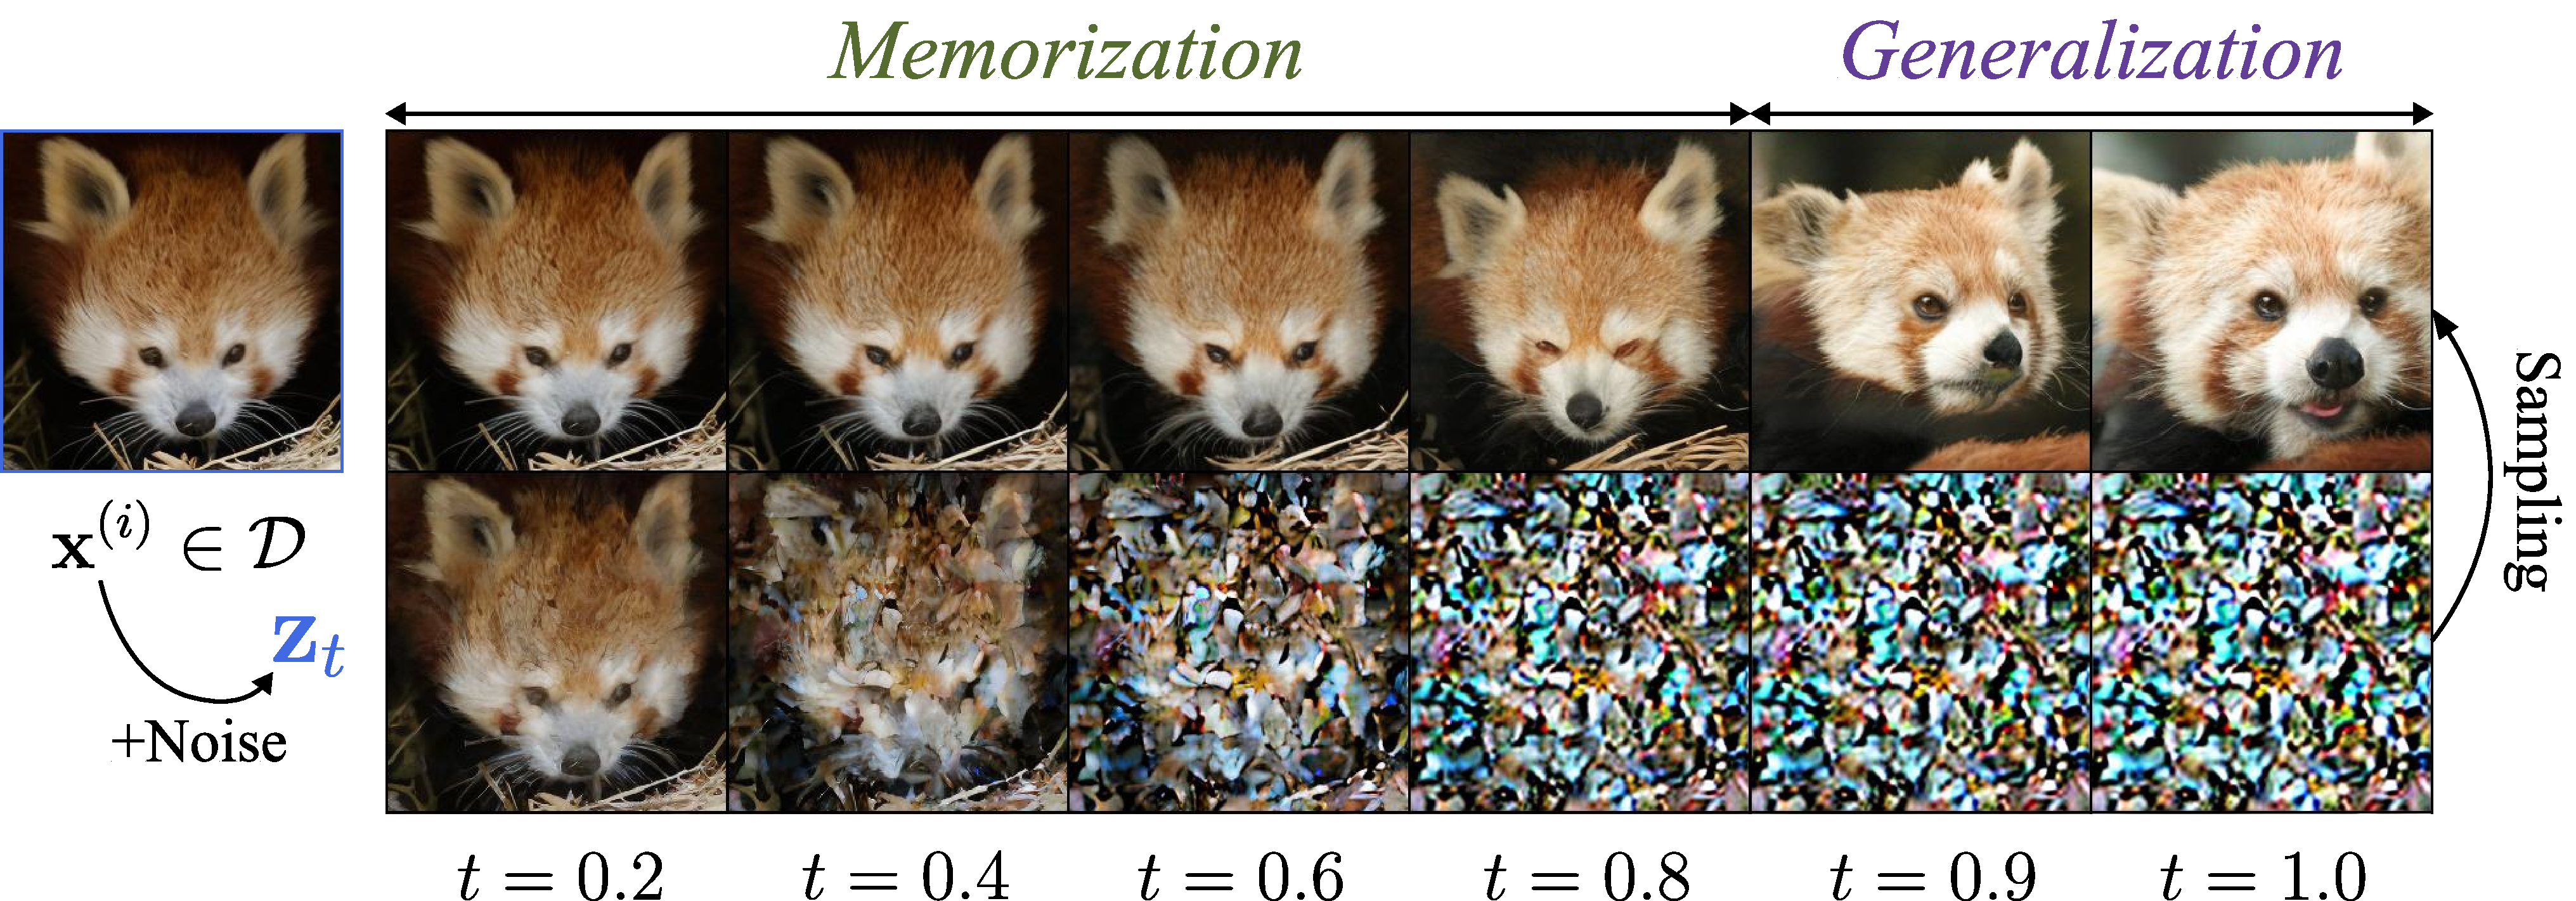
\includegraphics[width=\textwidth]{figures/generalization/phase_transition_example}
    \end{subfigure}
    \hfill
    \begin{subfigure}[t]{0.29\textwidth}
        \centering
        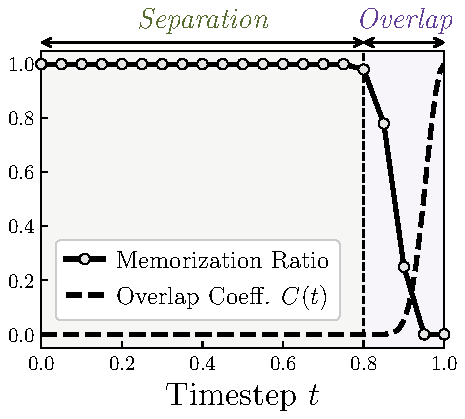
\includegraphics[width=\textwidth,trim=0 0.55cm 0 0]{figures/generalization/phase_transition_plot}
    \end{subfigure}
        \caption{\textbf{Qualitative example of selective underfitting.} \emph{Left}: Sampling ($t \to 0$) from a noisy image $\xblue{\rvz_t}$ in the supervision region maps back to the original training image $\rvx^{(i)}$ for most time steps ($t < 0.8$). \emph{Right}: The overlap coefficient $C(t)$ and memorization ratio. The \coloredul{black}{memorization ratio} exhibits the same trend quantitatively.}
    \label{fig:phase-transition}
    \venueifelse{\vskip -1.5\baselineskip}{\vskip -0.5\baselineskip}
\end{tmpfigure}